%This file is encoded in UTF-8 and requires XeLaTeX to compile.

%\documentclass[12pt,a4paper]{report}
\documentclass[10pt,a4paper]{scrartcl} %for \subtitle{} macro
%\usepackage[paperwidth=95mm, paperheight=120mm, margin=2mm]{geometry}%设置页面的长宽和边距。 % 6'
%\usepackage[paperwidth=210mm, paperheight=297mm, margin=25mm]{geometry}%设置页面的长宽和边距。 % A4
\usepackage[paperwidth=355mm, paperheight=188mm, margin=30mm]{geometry}%设置页面的长宽和边距。 % apple mac air 13' with adobe reader
\usepackage[utf8]{inputenc}
\usepackage[english]{babel}
\usepackage{amsmath,amsthm}
\usepackage[utopia]{mathdesign}
\usepackage{xunicode,xltxtra}
\usepackage{url}
\usepackage{color}
\usepackage[usenames,dvipsnames,svgnames,table]{xcolor}
\usepackage{makeidx}
\usepackage{graphics}
\usepackage{graphicx}
\usepackage{float}
\usepackage{sidecap}
\usepackage{longtable}
\usepackage[font=small,labelfont=bf]{caption}
\usepackage{lastpage}                                           
\usepackage{layout} 
\usepackage{fancyhdr}

\makeatletter
\defaultfontfeatures{Mapping=tex-text}
%\setmainfont{DejaVu Serif}
%\setsansfont[BoldFont={DejaVu Sans Condensed}]{DejaVu Sans Condensed}
%\setmonofont[BoldFont={DejaVu Sans Mono}]{DejaVu Sans Mono}
\setmainfont[BoldFont=Adobe Garamond Pro Bold,ItalicFont=Apple Chancery]{Adobe Garamond Pro}
\setmonofont{Andale Mono}
%\floatstyle{boxed} 
%\restylefloat{figure}
\graphicspath{{./doc/figure/}}
\renewcommand{\thefootnote}{\fnsymbol{footnote}}    
\makeatother
\usepackage{fontspec}
\setlength{\parskip}{8pt}
\setlength{\parindent}{0mm}
\frenchspacing

\pagestyle{fancy}

%Shortcuts for font family selection.
\newcommand{\rmf}{\rmfamily}
\newcommand{\sff}{\sffamily}
\newcommand{\ttf}{\ttfamily}
\newcommand{\trm}{\textrm}
\newcommand{\tsf}{\textsf}
\newcommand{\ttt}{\texttt}
\newcommand{\tb}{\textbf}
\newcommand{\ti}{\textit}
\newcommand{\tbi}[1]{\textbf{\textit{#1}}}

\definecolor{codeback1}{gray}{0.85}
\definecolor{codeback2}{gray}{0.95}

\title{Variate Generator Library}
\subtitle{User's Guide}
\author{Feng Wang\\feng.wang@uni-ulm.de}

\makeindex

\begin{document}

\maketitle
\newpage

\tableofcontents
\newpage

\section{Getting Started}

\subsection{Welcome}

Welcome to Variate Generator library! 

By the time you have read through this tutorial, you will be able to play with it.

\subsection{Compilation Enviroment Requirement}

As some C++11\footnote{Features such as lambda functions, variadic template and keyword auto, see http://www.open-std.org/jtc1/sc22/wg21/ for more information.} features are employed when implementing this library, 
before we get further, please check your compiler for C++11 compatablity.

\subsection{A Quick Example}

The code listed in Table \ref{code:gauss} shows how to generate gaussian random numbers:

\begin{small}
\begin{ttfamily}

\begin{center}
\rowcolors{1}{codeback1}{codeback2}
%\rowcolors{1}{White}{Silver}
%\begin{tabular}{|l|}
\begin{longtable}{|l|}
\caption{Source Code for a Gaussian Variate Example} \\
\label{code:gauss} \\
%%code
\hline
%\noindent
\mbox{}\textbf{\textcolor{RoyalBlue}{\#include}}\ \texttt{\textcolor{Red}{\textless{}vg.hpp\textgreater{}}} \\
%\mbox{} \\
\mbox{}\textbf{\textcolor{RoyalBlue}{\#include}}\ \texttt{\textcolor{Red}{\textless{}cmath\textgreater{}}} \\
\mbox{}\textbf{\textcolor{RoyalBlue}{\#include}}\ \texttt{\textcolor{Red}{\textless{}map\textgreater{}}} \\
\mbox{}\textbf{\textcolor{RoyalBlue}{\#include}}\ \texttt{\textcolor{Red}{\textless{}iostream\textgreater{}}} \\
%\mbox{} \\
\mbox{}\textcolor{ForestGreen}{int}\ \textbf{\textcolor{Black}{main}}\textcolor{BrickRed}{()} \\
\mbox{}\textcolor{Red}{\{} \\
\mbox{}\ \ \ \ \textit{\textcolor{Gray}{//generate\ double\ precision\ gaussian\ random\ numbers}} \\
\mbox{}\ \ \ \ \textit{\textcolor{Gray}{//using\ mt19937\ as\ random\ generator\ engine\ with\ arguments\ (0,4)}} \\
\mbox{}\ \ \ \ vg\textcolor{BrickRed}{::}\textcolor{TealBlue}{variate$\_$generator\textless{}double,\ vg::gaussian,\ vg::mt19937\textgreater{}}\ \textbf{\textcolor{Black}{vg}}\textcolor{BrickRed}{(}\textcolor{Purple}{0}\textcolor{BrickRed}{,}\ \textcolor{Purple}{4}\textcolor{BrickRed}{);}\ \ \ \  \\
\mbox{}\ \ \ \ std\textcolor{BrickRed}{::}\textcolor{TealBlue}{map\textless{}\ int,\ int\ \textgreater{}}\ sample\textcolor{BrickRed}{;} \\
%\mbox{} \\
\mbox{}\ \ \ \ \textit{\textcolor{Gray}{//generate\ 500\ gaussian\ numbers\ and\ store\ them\ in\ a\ map}} \\
\mbox{}\ \ \ \ \textbf{\textcolor{Blue}{for}}\ \textcolor{BrickRed}{(}\ \textbf{\textcolor{Blue}{auto}}\ i\ \textcolor{BrickRed}{=}\ vg\textcolor{BrickRed}{.}\textbf{\textcolor{Black}{begin}}\textcolor{BrickRed}{();}\ i\ \textcolor{BrickRed}{!=}\ vg\textcolor{BrickRed}{.}\textbf{\textcolor{Black}{begin}}\textcolor{BrickRed}{()+}\textcolor{Purple}{500}\textcolor{BrickRed}{;}\ \textcolor{BrickRed}{++}i\ \textcolor{BrickRed}{)} \\
\mbox{}\ \ \ \ \ \ \ \ sample\textcolor{BrickRed}{[}std\textcolor{BrickRed}{::}\textbf{\textcolor{Black}{round}}\textcolor{BrickRed}{(*}i\textcolor{BrickRed}{)]++;} \\
%\mbox{} \\
\mbox{}\ \ \ \ \textit{\textcolor{Gray}{//show\ the\ number\ generated}} \\
\mbox{}\ \ \ \ \textbf{\textcolor{Blue}{for}}\ \textcolor{BrickRed}{(}\ \textbf{\textcolor{Blue}{auto}}\ i\ \textcolor{BrickRed}{=}\ sample\textcolor{BrickRed}{.}\textbf{\textcolor{Black}{begin}}\textcolor{BrickRed}{();}\ i\ \textcolor{BrickRed}{!=}\ sample\textcolor{BrickRed}{.}\textbf{\textcolor{Black}{end}}\textcolor{BrickRed}{();}\ \textcolor{BrickRed}{++}i\ \textcolor{BrickRed}{)} \\
\mbox{}\ \ \ \ \textcolor{Red}{\{} \\
\mbox{}\ \ \ \ \ \ \ \ std\textcolor{BrickRed}{::}cout\ \textcolor{BrickRed}{\textless{}\textless{}}\ \textcolor{BrickRed}{(*}i\textcolor{BrickRed}{).}first\ \textcolor{BrickRed}{\textless{}\textless{}}\ \texttt{\textcolor{Red}{"{}}}\texttt{\textcolor{CarnationPink}{\textbackslash{}t}}\texttt{\textcolor{Red}{"{}}}\textcolor{BrickRed}{;} \\
\mbox{}\ \ \ \ \ \ \ \ \textbf{\textcolor{Blue}{for}}\ \textcolor{BrickRed}{(}\ \textbf{\textcolor{Blue}{auto}}\ j\ \textcolor{BrickRed}{=}\ \textcolor{Purple}{0}\textcolor{BrickRed}{;}\ j\ \textcolor{BrickRed}{\textless{}}\ \textcolor{BrickRed}{(*}i\textcolor{BrickRed}{).}second\textcolor{BrickRed}{;}\ \textcolor{BrickRed}{++}j\ \textcolor{BrickRed}{)} \\
\mbox{}\ \ \ \ \ \ \ \ \ \ \ \ std\textcolor{BrickRed}{::}cout\ \textcolor{BrickRed}{\textless{}\textless{}}\ \texttt{\textcolor{Red}{"{}*"{}}}\textcolor{BrickRed}{;} \\
\mbox{}\ \ \ \ \ \ \ \ std\textcolor{BrickRed}{::}cout\ \textcolor{BrickRed}{\textless{}\textless{}}\ \texttt{\textcolor{Red}{"{}}}\texttt{\textcolor{CarnationPink}{\textbackslash{}n}}\texttt{\textcolor{Red}{"{}}}\textcolor{BrickRed}{;} \\
\mbox{}\ \ \ \ \textcolor{Red}{\}} \\
%\mbox{} \\
\mbox{}\ \ \ \ \textbf{\textcolor{Blue}{return}}\ \textcolor{Purple}{0}\textcolor{BrickRed}{;} \\
\mbox{}\textcolor{Red}{\}} \\
%\mbox{} \\
%\mbox{}
\hline
%\end{tabular}
\end{longtable}
\end{center}

\end{ttfamily}
\end{small}

As this library is header file only,
if your c++ compiler is g++, a typical compilation and link command for the example code whose file name is \textit{test\_gaussian.cc} can be

\begin{center}
\fcolorbox{White}{Silver}{\textcolor{Sepia}{\textbf{g++ -I\textit{PATH\_TO\_THE\_HEADER} -o ./bin/gaussian\_test test\_gaussian.cc -std=c++11 -Wall}}}
\end{center}

This command will generate a executable file \textit{test\_gaussian} in directory \textit{./bin}, 
and its executation result is shown in figure \ref{fig:gaussian}

\begin{figure}
\centering
\fbox{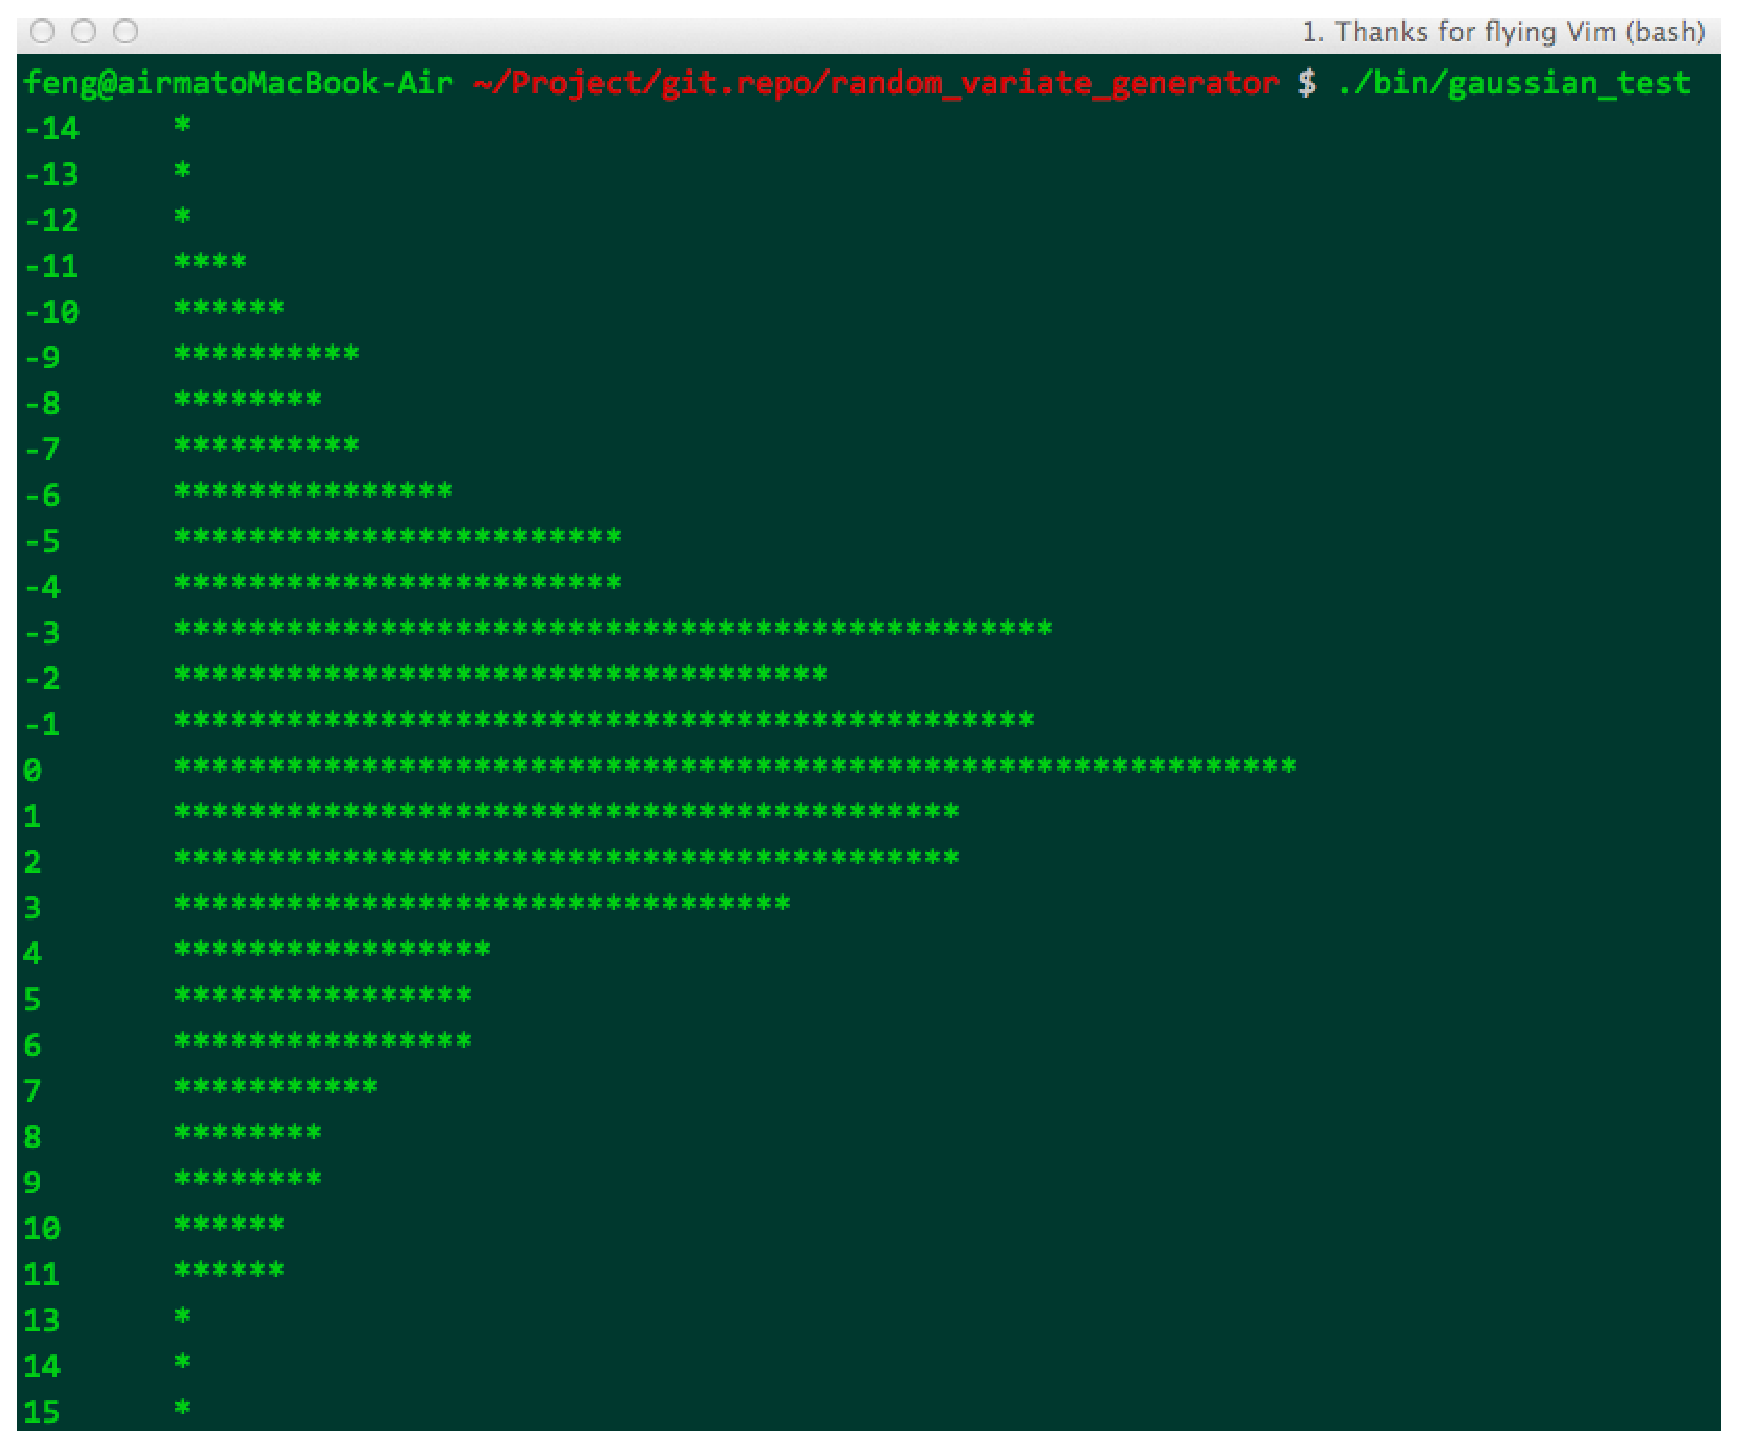
\includegraphics[scale=0.4]{gauss}}
\caption{Gaussian Random Number Example}
\label{fig:gaussian}
\end{figure}

%%code









\section{An Overview of VG}

A random variate generator consists of three parts:
%\begin{description}
%\begin{enumerate}
\begin{itemize}
    \item   variate type
    \item   distribution type
    \item   engine type
\end{itemize}
%\end{enumerate}
%\end{description}


\subsection{struct variate\_generator}


The basic struct used for a generator is variate\_generator, which is decleared as:

\begin{small}
\begin{ttfamily}

\begin{center}
\rowcolors{1}{codeback1}{codeback2}
%\rowcolors{1}{White}{Silver}
%\begin{tabular}{|l|}
\begin{longtable}{|l|}
\caption{variate\_generator struct} \\
\label{code:variate_generator} \\
%%code
\hline
\mbox{}\textbf{\textcolor{Blue}{namespace}}\ vg \\
\mbox{}\textcolor{Red}{\{} \\
\mbox{}\ \ \ \ \textbf{\textcolor{Blue}{template}} \\
\mbox{}\ \ \ \ \textcolor{BrickRed}{\textless{}}\ \ \  \\
\mbox{}\ \ \ \ \ \textbf{\textcolor{Blue}{class}}\ \textcolor{TealBlue}{T}\ \textcolor{BrickRed}{=}\ \textcolor{ForestGreen}{double}\textcolor{BrickRed}{,}\ \ \ \ \ \ \ \ \ \ \ \ \ \ \ \ \ \ \ \ \ \ \ \ \ \ \ \ \ \ \ \ \ \ \ \textit{\textcolor{Brown}{//variate}} \\
\mbox{}\ \ \ \ \ \textbf{\textcolor{Blue}{template}}\textcolor{BrickRed}{\textless{}}\textbf{\textcolor{Blue}{class}}\textcolor{BrickRed}{,}\ \textbf{\textcolor{Blue}{class}}\textcolor{BrickRed}{\textgreater{}}\ \textbf{\textcolor{Blue}{class}}\ \textcolor{TealBlue}{Distribution}\ \textcolor{BrickRed}{=}\ uniform\textcolor{BrickRed}{,}\textit{\textcolor{Brown}{//distribution}} \\
\mbox{}\ \ \ \ \ \textbf{\textcolor{Blue}{class}}\ \textcolor{TealBlue}{Engine}\ \textcolor{BrickRed}{=}\ mitchell$\_$moore\ \ \ \ \ \ \ \ \ \ \ \ \ \ \ \ \ \ \ \ \ \ \ \textit{\textcolor{Brown}{//engine\ }} \\
\mbox{}\ \ \ \ \textcolor{BrickRed}{\textgreater{}} \\
\mbox{}\ \ \ \ \textbf{\textcolor{Blue}{struct}}\ \textcolor{TealBlue}{variate$\_$generator} \\
\mbox{}\ \ \ \ \textcolor{Red}{\{} \\
\mbox{}\ \ \ \ \ \ \ \textbf{\textcolor{Blue}{template}}\textcolor{BrickRed}{\textless{}}\ \textbf{\textcolor{Blue}{typename}}\ \textcolor{BrickRed}{...}\ Tn\ \textcolor{BrickRed}{\textgreater{}} \\
\mbox{}\ \ \ \ \ \ \ \textbf{\textcolor{Black}{variate$\_$generator}}\textcolor{BrickRed}{(}\ \textbf{\textcolor{Blue}{const}}\ Tn\ \textcolor{BrickRed}{...}\ \textcolor{BrickRed}{);} \\
\mbox{}\ \ \ \ \ \ \ \textcolor{TealBlue}{T}\ \textbf{\textcolor{Blue}{operator}}\textcolor{BrickRed}{()()}\ \textbf{\textcolor{Blue}{const}}\textcolor{BrickRed}{;}\  \\
\mbox{}\ \ \ \ \ \ \ \textbf{\textcolor{Blue}{operator}}\ \textbf{\textcolor{Black}{T}}\textcolor{BrickRed}{()}\ \textbf{\textcolor{Blue}{const}}\textcolor{BrickRed}{;} \\
\mbox{}\ \ \ \ \ \ \ \textcolor{TealBlue}{iterator}\ \textbf{\textcolor{Black}{begin}}\textcolor{BrickRed}{()}\ \textbf{\textcolor{Blue}{const}}\textcolor{BrickRed}{;} \\
\mbox{}\ \ \ \ \textcolor{Red}{\}}\textcolor{BrickRed}{;} \\
\mbox{}\textcolor{Red}{\}}\textcolor{BrickRed}{;} \\
\hline
\end{longtable}
\end{center}

\end{ttfamily}
\end{small}

\subsubsection{declaration}

So to make a generator to product variates of int type and lagarithmic distribution, with a parameter 0.33, we can simply declare:

\noindent
\mbox{}vg\textcolor{BrickRed}{::}\textcolor{TealBlue}{variate$\_$generator\textless{}int,\ vg::lagarithmic\textgreater{}}\ \textbf{\textcolor{Black}{v}}\textcolor{BrickRed}{(}\ \textcolor{Purple}{0.33}\ \textcolor{BrickRed}{);} \\
\mbox{}

which it is equivalent to 

\noindent
\mbox{}vg\textcolor{BrickRed}{::}\textcolor{TealBlue}{variate$\_$generator\textless{}int,\ vg::lagarithmic,\ vg::mitchell$\_$moore\textgreater{}}\ \textbf{\textcolor{Black}{v}}\textcolor{BrickRed}{(}\ \textcolor{Purple}{0.33}\textcolor{BrickRed}{,}\ \textcolor{Purple}{0}\ \textcolor{BrickRed}{);} \\
\mbox{}

where the last argument 0 is the default engine seed.

Also, to make a generator to product variates of hypergeometric distribution, with int type and paramenters (200, 200, 200), using mt19937 persudo--random engine and engine seed 987654321, we can declare it with one line code like this:

\noindent
\mbox{}vg\textcolor{BrickRed}{::}\textcolor{TealBlue}{variate$\_$generator\textless{}int,\ vg::hypergeometric,\ vg::mt19937\textgreater{}}\ \textbf{\textcolor{Black}{v}}\textcolor{BrickRed}{(}\ \textcolor{Purple}{200}\textcolor{BrickRed}{,}\ \textcolor{Purple}{200}\textcolor{BrickRed}{,}\ \textcolor{Purple}{200}\textcolor{BrickRed}{,}\ \textcolor{Purple}{987654321}\ \textcolor{BrickRed}{);} \\
\mbox{}

\subsubsection{Generation}

After the generator $v$ has been declared, we can generate variate in several ways:

%\begin{description}
%    \item[One Variate] \\
                        %\noindent

                        Generate only one variate: 

                        \noindent
                        \mbox{}\textbf{\textcolor{Blue}{auto}}\ i\ \textcolor{BrickRed}{=}\ \textbf{\textcolor{Black}{v}}\textcolor{BrickRed}{();} \\
                        \mbox{}\textcolor{ForestGreen}{int}\ j\ \textcolor{BrickRed}{=}\ v\textcolor{BrickRed}{;} \\
                        \mbox{}\textbf{\textcolor{Blue}{auto}}\ k\ \textcolor{BrickRed}{=}\ \textcolor{BrickRed}{*(}v\textcolor{BrickRed}{.}\textbf{\textcolor{Black}{begin}}\textcolor{BrickRed}{());} \\
                        \mbox{}
%    \item[Multiple Variates] \\

                        Generate multiple variates: 

                        \noindent
                        \mbox{}std\textcolor{BrickRed}{::}\textcolor{TealBlue}{vector\textless{}int\textgreater{}}\ \textbf{\textcolor{Black}{array1}}\textcolor{BrickRed}{(}\ v\textcolor{BrickRed}{.}\textbf{\textcolor{Black}{begin}}\textcolor{BrickRed}{(),}\ v\textcolor{BrickRed}{.}\textbf{\textcolor{Black}{begin}}\textcolor{BrickRed}{()+}\textcolor{Purple}{100}\textcolor{BrickRed}{);} \\
                        \mbox{}std\textcolor{BrickRed}{::}\textcolor{TealBlue}{vector\textless{}int\textgreater{}}\ \textbf{\textcolor{Black}{array2}}\textcolor{BrickRed}{(}\ \textcolor{Purple}{100}\ \textcolor{BrickRed}{);}\  \\
                        \mbox{}std\textcolor{BrickRed}{::}\textbf{\textcolor{Black}{generate}}\textcolor{BrickRed}{(}\ array2\textcolor{BrickRed}{.}\textbf{\textcolor{Black}{begin}}\textcolor{BrickRed}{(),}\ array2\textcolor{BrickRed}{.}\textbf{\textcolor{Black}{end}}\textcolor{BrickRed}{(),}\ v\ \textcolor{BrickRed}{);} \\
                        \mbox{}std\textcolor{BrickRed}{::}\textcolor{TealBlue}{vector\textless{}int\textgreater{}}\ array3\textcolor{BrickRed}{;}\  \\
                        \mbox{}std\textcolor{BrickRed}{::}\textbf{\textcolor{Black}{copy}}\textcolor{BrickRed}{(}\ v\textcolor{BrickRed}{.}\textbf{\textcolor{Black}{begin}}\textcolor{BrickRed}{(),}\ v\textcolor{BrickRed}{.}\textbf{\textcolor{Black}{begin}}\textcolor{BrickRed}{()+}\textcolor{Purple}{100}\textcolor{BrickRed}{,}\ std\textcolor{BrickRed}{::}\textbf{\textcolor{Black}{back$\_$inserter}}\textcolor{BrickRed}{(}\ array3\ \textcolor{BrickRed}{)}\ \textcolor{BrickRed}{);} \\
                        \mbox{}

%\end{description}

\subsection{Built-in Distributions}

Curent we have more than fifty distributions implemented:
\begin{itemize}
    \item arcsine distribution \ref{arcsinedistribution}
    \item balding nichols distribution
    \item bernoulli distribution
    \item beta distribution
    \item beta\_binomial distribution
    \item beta\_pascal distribution
    \item binomial distribution
    \item burr distribution
    \item cauchy distribution
    \item chi\_square distribution
    \item digamma distribution
    \item erlang distribution
    \item exponential distribution
    \item exponential\_power distribution
    \item extreme\_value distribution
    \item f distribution
    \item factorial distribution
    \item gamma distribution
    \item gaussian distribution
    \item gaussian\_tail distribution
    \item generalized\_hypergeometric\_b3 distribution
    \item generalized\_waring distribution
    \item geometric distribution
    \item grassia distribution
    \item gumbel\_1 distribution
    \item gumbel\_2 distribution
    \item hyperbolic\_secant distribution
    \item hypergeometric distribution
    \item inverse\_gaussian distribution
    \item inverse\_polya\_eggenberger distribution
    \item lambda distribution
    \item laplace distribution
    \item levy distribution
    \item list distribution
    \item logarithmic distribution
    \item logistic distribution
    \item lognormal distribution
    \item mizutani distribution
    \item negative\_binomial distribution
    \item negative\_binomial\_beta distribution
    \item normal distribution
    \item pareto distribution
    \item pascal distribution
    \item pearson distribution
    \item planck distribution
    \item poisson distribution
    \item polya distribution
    \item polya\_aeppli distribution
    \item rayleigh distribution
    \item rayleigh\_tail distribution
    \item singh\_maddala distribution
    \item t distribution
    \item teichroew distribution
    \item triangular distribution
    \item trigamma distribution
    \item uniform distribution \ref{uniformdistribution}
    \item von\_mises distribution
    \item wald distribution
    \item waring distribution
    \item weibull distribution
    \item yule distribution
    \item zipf distribution
\end{itemize}

\subsection{Engines}
Currently we have 3 engines implemented:
\begin{itemize}
    \item linear\_congruential
    \item mitchell\_moore
    \item mt19937
\end{itemize}










\end{document}
